\newcommand{\usecase}[8]{
\begin{table}
    \centering
    \begin{tabular}{|l|}
        \hline
        \textbf{Identifikator}: #1\\
        \hline
        \textbf{Naziv}: #2\\
        \hline
        \textbf{Učesnik}: #3\\
        \hline
        \textbf{Opis}: #4\\
        \hline
        \textbf{Preduslovi}: #5\\
        \hline
        \textbf{Posledice}: #6\\
        \hline
        \textbf{Osnovni tok izvršavanja}\\
        \begin{minipage}{0.9\textwidth}
            \vskip 4pt
            \begin{enumerate}
                #7
            \end{enumerate}
            \vskip 4pt
        \end{minipage}\\
        \hline
        #8
    \end{tabular}
    \caption{#2}
\end{table}
}

\newcommand{\altflow}[2]{
    \textbf{Alternativni tok #1}\\
    \begin{minipage}{0.9\textwidth}
        \vskip 4pt
        \begin{enumerate}
            #2
        \end{enumerate}
        \vskip 4pt
    \end{minipage}\\
    \hline
}

\rhead{4. Dijagram slučajeva korišćenja}
\section{Dijagram slučajeva korišćenja}
U nastavku se nalazi dijagram slučajeva korišćenja [Slika \ref{fig:use-case}] na kome su prikazane pravila poslovanja.
\begin{figure}[h]
    \centering
    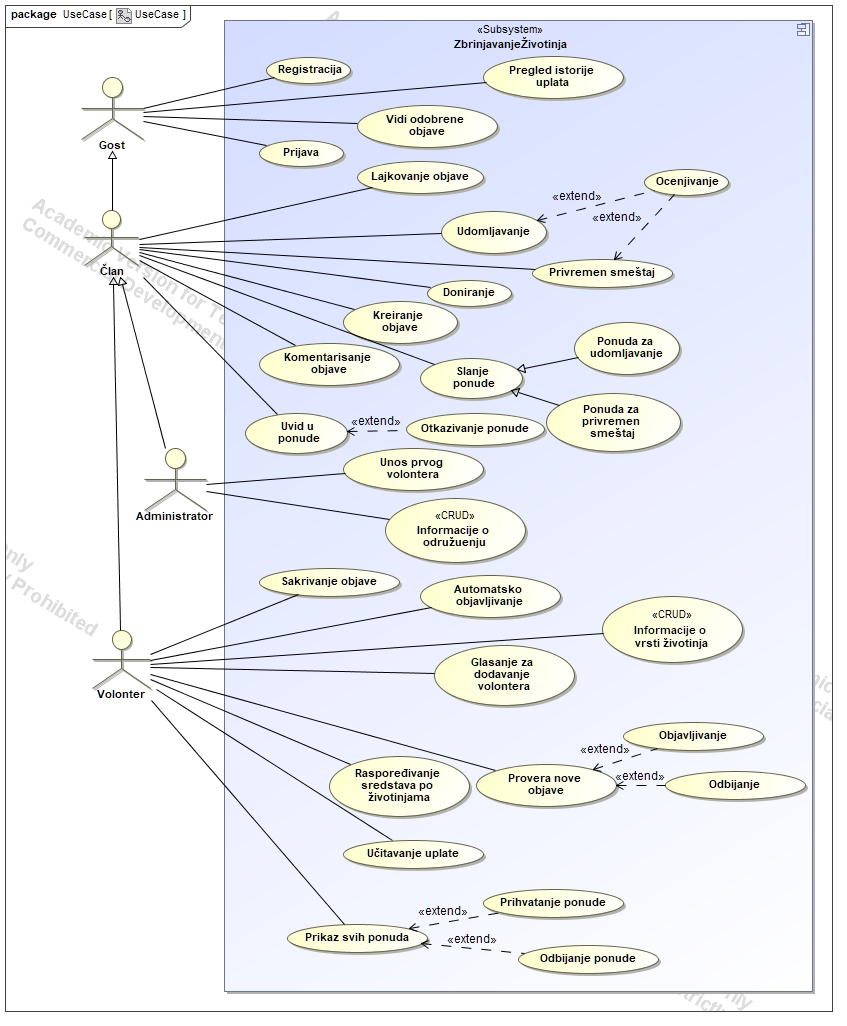
\includegraphics[width=\textwidth]{img/use-case.jpg}
    \caption{Dijagram slučajeva korišćenja}
    \label{fig:use-case}
\end{figure}
\subsection{Specifikacija slučajeva korišćenja}
\par U nastavku se nalaze specifikacija korišćenja prikazani na dijagramu slučajeva korišćenja [Slika \ref{fig:use-case}].
\usecase{GI1}
        {Registracija}
        {Gost}
        {Gost se registruje na sistem}
        {Otvorena registraciona forma}
        {Gost ima mogućnost da se prijavi na sistem}
        {
            \item Gost unosi ime, prezime, adresu, datum rođenja, pol i broj telefona.
            \item Sistem proverava validnost podataka.
            \item Sistem obaveštava gosta da je registracija prošla uspešno. [Alternativni tok A]
            \item Kraj scenarija.
        }
        {
            \altflow{A: Neispravno uneti podaci}
            {
                \item Sistem obaveštava gosta o greškama u formi.
                \item Prikazuje se forma za registraciju.
                \item Kraj scenarija.
            }
        }
\usecase{GI2}
          {Vidi odobrene objave}
          {Gost}
          {Prikaz odobrenih objava gostu}
          {Nema preduslova}
          {Član može da vidi odobrene objave}
          {
            \item Sistem učitava sve odobrene objave.
            \item Kraj scenarija.
          }
          {}

\usecase{GI3}
         {Pregled istorije donacija}
         {Gost}
         {Prikaz svih prethodnih donacija}
         {Pritisnuto je dugme za prikaz istorije donacija}
         {član može da vidi sve prethodne donacije}
         {
            \item Sistem učitava istoriju donacija.
            \item Kraj scenarija
         }
         {}


\usecase{GI4}
        {Prijava}
        {Gost}
        {Prijava člana na sistem unosom korisničkog imena i šifre}
        {Otvorena je forma za prijavu}
        {Član može da koristi funkcionalnosti sistema}
        {
            \item Gost unosi korisničko ime i šifru.
            \item Sistem proverava da li su korisničko ime i šifra ispravni.
            \item Sistem otvara odgovarajući meni [Alternativni tok A]
            \item Kraj scenarija.
        }
        {
            \altflow{A: Neispravno korisničko ime ili šifra}
            {
                \item Sistem obaveštava gosta da su korisničko ime ili šifra neispravni.
                \item Gost potvrđuje da je video obaveštenje.
                \item Prikazuje se forma za prijavu.
                \item Kraj scenarija.
            }
        }

\usecase{MI1}
         {Doniranje}
         {Član}
         {Prikaz informacija za donacije}
         {\makecell[l]{Član je prijavljen na sistem i dugme za donacije \\je pritisnuto}}
         {Član ima informacije potrebne za slanje donacije}
         {
            \item Sistem prikazuje informacije o bankovnom računu
            \item Kraj scenarija
         }
         {}

\usecase{MI2}
         {Zahtev za promociju u volontera}
         {Član}
         {Član šalje zahtev za promociju u volontera}
         {Član je prijavljen na sitem}
         {Zahtev je zabeležen u sistemu}
         {
            \item Član podnosi zahtev za promociju.
            \item Sistem obaveštava člana da je zahtev uspešno poslat.
            \item Sistem trajno čuva zahtev.
            \item Kraj scenarija.
         }{}

\usecase{MI3}
         {Označava objavu da mu se sviđa}
         {Član}
         {Član označava objavu da mu se sviđa}
         {Član je prijavljen na sistem}
         {Promenjen broj sviđanja na objavi}
         {
            \item Sistem vizuelno obaveštava člana da mu se objava sviđa.
            \item Sistem dodaje člana u listu sviđanja za objavu.[Alternativni tok A]
            \item Kraj scenarija.
         }
         {
            \altflow{A: Član je već označio da mu se objava sviđa}
            {
                \item Sistem uklanja člana iz liste sviđanja za objavu.
                \item Kraj scenarija.
            }
         }

\usecase{MI4}
         {Komentarisanje objave}
         {Član}
         {Član komentariše objavu}
         {Član je prijavljen na sistem}
         {Dodat novi komentar na objavu}
         {
            \item Član unosi komentar.
            \item Sistem dodaje komentar na objavu.
            \item Kraj scenarija.
         }
         {}

\usecase{MI5}
         {Uvid u ponude}
         {Član}
         {\makecell[l]{Član ima uvid u sve njehgve ponude. EP1 Član otkazuje \\ponudu. EP2 Član ostavlja ocenu}}
         {\makecell[l]{Član je prijavljen na sistem. Pritisnuto je dugme\\ za prikaz ponuda}}
         {Članova odluka se trajno čuva}
         {
            \item Sistem prikazuje sve njegove ponude.
            \item $[$Tačka proširenja: EP1 Otkazivanje ponude$]$ $[$Tačka proširenja: EP2 Ocenjivanje$]$
            \item Kraj scenarija.
         }
         {}

\usecase{EP1}
        {Otkazivanje ponude}
        {Član}
        {Otkazivanje članove ponude}
        {Otvoren je prikaz članovih ponuda}
        {Članova odluka se trajno čuva}
        {
            \item Član aktivira brisanje ponude.
            \item Sistem obaveštava člana o posledicama otkazivanja.
            \item Član pritiska dugme otkaži. [Alternativni tok A]
            \item Sistem briše ponudu iz sistema i osvežava meni sa ponudama.
            \item Kraj scenarija.
        }
        {
            \altflow{A: Član odustaje od brisanja}
            {
                \item Sistem osvežava meni sa ponudama.
                \item Kraj scenarija.
            }
        }
        
\usecase{EP2}
        {Ocenjivanje}
        {Član}
        {Ocenjivanje ponude}
        {Otvoren je prikaz članovih ponuda}
        {Članova odluka se trajno čuva}
        {
            \item Član aktivira ocenjivanje ponude.
            \item Član unosi ocenu i komentar.
            \item Sistem čuva recenziju i osvežava meni sa ponudama.
            \item Kraj scenarija.
        }
        {}
        
\usecase{MI6}
        {Kreiranje objave}
        {Član}
        {Član kreira ponudu}
        {Član je prijavljen na sistem}
        {Nova objava je dodata u sistem}
        {
            \item Član aktivira kreiranje objave.
            \item Član popunjava formu odgovarajućim podacima.
            \item Sistem kreira objavu. 
            \item Sistem inicijalizuje objavu.
            \item Kraj scenarija.
        }
        {}
        
\usecase{MI7}
        {Privremen smeštaj}
        {Član}
        {Član pruža privremen smeštaj}
        {\makecell[l]{Član je prijavljen na sistem i poslao je ponudu za \\privremen smeštaj koja je prihvaćena}}
        {Životinja je dobila privremen smeštaj}
        {
            \item Član pregleda obaveštenje da mu je ponuda za privremen smeštaj prihvaćena.
            \item Član pruža životinji privremen smeštaj.
            \item Kraj scenarija.
        }
        {}
        
\usecase{MI8}
        {Udomljavanje}
        {Član}
        {Član udomljava životinju}
        {\makecell[l]{Član je prijavljen na sistem i poslao je ponudu za \\ udomljavanje koja je prihvaćena}}
        {Životinja je udomljena}
        {
            \item Član pregleda obaveštenje da mu je ponuda za udomljavanje prihvaćena.
            \item Član udomljava životinju.
            \item Kraj scenarija.
        }
        {}
        
\usecase{MI9}
        {Slanje ponude}
        {Član}
        {\makecell[l]{Član šalje ponudu. EP3 Član šalje ponudu za \\privremen smeštaj. EP4 Član šalje ponudu za udomljavanje}}
        {Član je prijavljen na sistem i otvoren je prikaz objava}
        {Poslata ponuda je zabeležena u sistemu}
        {
            \item $[$Tačka proširenja EP3 Ponuda za privremen smeštaj. EP4 Ponuda za udomljavanje $]$
            \item Kraj scenarija.
        }
        {}

\usecase{EP3}
        {Ponuda za privremen smeštaj}
        {Član}
        {Član šalje ponudu za privremen smeštaj}
        {Član je prijavljen na sistem i otvoren je prikaz objava}
        {Poslata ponuda je zabeležena u sistemu}
        {
            \item Član bira slanje ponude za privremen smeštaj.
            \item Sistem kreira ponudu.
            \item Sistem obaveštava korisnika o uspešno poslatoj ponudu.
            \item Kraj scenarija.
        }
        {}
        
\usecase{EP4}
        {Ponuda za udomljavanje}
        {Član}
        {Član šalje ponudu za udomljavanje}
        {Član je prijavljen na sistem i otvoren je prikaz objava}
        {Poslata ponuda je zabeležena u sistemu}
        {
            \item Član bira slanje ponude za udomljavanje.
            \item Sistem kreira ponudu.
            \item Sistem obaveštava korisnika o uspešno poslatoj ponudu.
            \item Kraj scenarija.
        }
        {}
        
\usecase{VI1}
        {Sakrivanje/Otkrivanje objave}
        {Volonter}
        {Volonter sakriva ili otkriva objavu}
        {Volonter je prijavljen na sistem i otvoren je prikaz objava}
        {Stanje objave je promenjeno}
        {
            \item Volonter pritiska dugme za sakrivanje/otkrivanje objave.
            \item Sistem menja stanje objave na Sakrivena. [Alternativni tok A]
            \item Sistem menja prikaz objave.
            \item Kraj scenarija.
        }
        {
            \altflow{A: Objava već ima stanje Sakrivena}
            {
                    \item Sistem menja stanje objave na Prihvaćena.
                    \item Sistem menja prikaz objave.
                    \item Kraj scenarija.
            }
        }
        
\usecase{VI2}
        {Glasanje za dodavanje volontera}
        {Volonter}
        {Volonter glasa za dodavanje volontera}
        {\makecell[l]{Volonter je prijavljen na sistem, otvoren je prikaz \\zahteva na čekanju i korisnik još uvek nije glasao na \\dati zahtev}}
        {Volonterov glas je zabeležen}
        {
            \item Volonter pritiska dugme za glasanje za ili protiv.
            \item Sistem beleži volonterov glas i ažurira zahtev.
            \item Sistem osvežava listu zahteva.
            \item Kraj scenarija.
        }
        {}
        
\usecase{VI3}
        {Provera nove objave}
        {Volonter}
        {Volonter proverava nove objave}
        {Volonter je prijavljen na sistem}
        {Stanje objave je promenjeno}
        {
            \item Sistem učitava sve nove objave.
            \item $[$Tačka proširenja EP5 Prihvatanje$]$ $[$Tačka proširenja EP6 Odbijanje$]$
            \item Kraj scenarija.
        }
        {}
        
\usecase{EP5}
        {Prihvatanje}
        {Volonter}
        {Volonter prihvata novu objavu}
        {\makecell[l]{Volonter je prijavljen na sistem i odabrana je objava \\ sa stanjem NaČekanju}}
        {Stanje objave je promenjeno}
        {
            \item Volonter pritiska dugme prihvatanja objave.
            \item Sistem menja stanje objave na Prihvaćena.
            \item Sistem menja prikaz objave.
            \item Kraj scenarija.
        }
        {}
        
\usecase{EP6}
        {Odbijanje}
        {Volonter}
        {Volonter odbija novu objavu}
        {\makecell[l]{Volonter je prijavljen na sistem i odabrana je objava \\ sa stanjem NaČekanju}}
        {Stanje objave je promenjeno}
        {
            \item Volonter pritiska dugme odbijanja objave.
            \item Sistem menja stanje objave na Odbijena.
            \item Sistem menja prikaz objave.
            \item Kraj scenarija.
        }
        {}
        
\usecase{VI4}
        {Raspoređivanje sredstava po životinjama}
        {Volonter}
        {Volonter raspoređuje sredstva udruženja}
        {Volonter je prijavljen na sistem}
        {Raspored sredstava je ažuriran}
        {
            \item Sistem učitava listu životinja.
            \item Volonter menja vrednosti dodeljenjih sredstava za životnju.
            \item Sistem čuva promenu rasporeda sredstava.
            \item Kraj scenarija.
        }
        {}
        
\usecase{VI5}
        {Učitavanje uplate}
        {Volonter}
        {Volonter učitava uplatu}
        {Volonter je prijavljen na sistem}
        {Lista donacije je ažurirana}
        {
            \item Volonter pritiska dugme za učitavanje uplate.
            \item Volonter bira datoteku sa sadržajem uplate.
            \item Sistem ažurira listu donacija. [Alternativni tok A]
            \item Kraj scenarija.
        }
        {
            \altflow{A: Uplata je neispravna}
            {
                    \item Lista donacija ostaje nepromenjena.
                    \item Kraj scenarija.
            }
        }
        
\usecase{VI6}
        {Brisanje komentara}
        {Volonter}
        {Volonter briše komentar}
        {Volonter je prijavljen na sistem i otvoren je prikaz objava}
        {Komentar je obrisan}
        {
            \item Volonter pritiska dugme za brisanje komentara.
            \item Sistem briše komentar.
            \item Sistem ažurira objavu.
            \item Sistem osvežava prikaz objava.
            \item Kraj scenarija.
        }
        {}
        
\usecase{VI7}
        {Uvid u sve ponude}
        {Volonter}
        {Volonter dobija uvid u sve ponude}
        {Volonter je prijavljen na sistem}
        {Ponude su ažurirane}
        {
            \item Sistem učitava listu ponuda.
            \item $[$Tačka proširenja EP7 Prihvatanje ponude$]$ $[$Tačka proširenja EP8 Odbijanje ponude$]$
            \item Kraj scenarija.
        }
        {}

\usecase{EP7}
        {Prihvatanje ponude}
        {Volonter}
        {Volonter prihvata ponudu}
        {Volonter je prijavljen na sistem i otvoren je prikaz ponuda}
        {Promenjeno je stanje objave}
        {
            \item Volonter pritiska dugme za prihvatanje ponude. 
            \item Sistem šalje pošaljiocu ponude obaveštenje o uspehu i broj  autora objave.
            \item Sistem šalje autoru objave obaveštenje o uspehu i broj pošaljioca ponude.
            \item Sistem menja stanje objave.
            \item Sistem briše ponudu.
            \item Kraj scenarija.
        }
        {}
        
\usecase{EP8}
        {Odbijanje ponude}
        {Volonter}
        {Volonter odbija ponudu}
        {Volonter je prijavljen na sistem i otvoren je prikaz ponuda}
        {Promenjeno je stanje objave}
        {
            \item Volonter pritiska dugme za odbijanje ponude. 
            \item Sistem šalje pošaljiocu ponude obaveštenje o neuspehu.
            \item Sistem briše ponudu.
            \item Kraj scenarija.
        }
        {}
    
\usecase{AI1}
        {Unos prvog volontera}
        {Administrator}
        {Administrator unosi prvog volontera}
        {Administrator je prijavljen na sistem}
        {Volonter je dodat}
        {
            \item Administrator popunjava formu za dodavanje volontera.
            \item Sistem dodaje volontera u sistem.
            \item Kraj scenarija.
        }
        {}
        
\usecase{AI2}
        {Ažuriranje informacija o udruženju}
        {Administrator}
        {Administrator ažurira informacije o udruženju}
        {Administrator je prijavljen na sistem}
        {Informacije o udruženju su ažurirane}
        {
            \item Sistem učitava informacije u udruženju.
            \item Administrator menja željene informacije o udruženju.
            \item Sistem beleži promene.
            \item Kraj scenarija.
        }
        {}